\section{Motivation}
{Wenn heutzutage die Spezifikation eines Projektes in englischer Sprache formuliert wird, ist diese Spezifikation von Anfang an mehrdeutig, behauptet Jeannette Wing, Coperate Vice President von Microsoft Research. Des Weiteren sagt sie, dass jede natürliche Sprache mehrdeutig ist. Hingegen in formalen Spezifikationen, wird mathematisch präzise erklärt, was genau ein Programm machen soll.}\cite{WING01:FV}
\\
\\
Diese Seminararbeit soll einen tieferen Einblick in den Themenbereich der Programmcodeverifikation schaffen. Dabei wird sowohl auf die Grundlagen als auch technisch-detaillierte Beispiele eingegangen. Als Programmiersprache wird hierfür der Proof-Assistent Coq verwendet.


\section{Relevanz formaler Verifikation}
Es existieren unzählige Beispiele für die Relevanz von formaler Verifikation. Jeder Computer besteht beispielsweise aus vielen elektronischen Hardwareteilen wie Prozessoren, Grafikkarte et cetera. Zur Benutzung wird eine Hardware Description Language (HDL) eingesetzt, welche sowohl die Struktur als auch das Verhalten der elektronischen Bauteile beschreibt. Falls eine Firma nun einen Computer mit einer fehlerhaften HDL-Software verkauft, kann dies gravierende Folgen nach sich ziehen.
Daher ist es wichtig, dass sowohl die Bauteile als auch das Zusammenspiel von Hardware und Software ausgiebig getestet werden.\\
\\
Heutzutage gehen die meisten Computer-Nutzer davon aus, dass ein Betriebssystem, ein Compiler oder andere Software zu 100\% korrekt funktionieren. Doch wie ist sichergestellt, dass das Speichern in einem Editor oder das Compilieren von C Code auch in jedem Fall das gewünschte Ergebnis liefert? \\
Sehr wahrscheinlich wurden viele verschiedene Tests bereits vor der Veröffentlichung der jeweiligen Software durchgeführt. Die bekanntesten sind Unit-, Integration- und manuelle Tests. Dabei versucht man sowohl Standard- als auch Grenz- und Sonderfälle abzudecken, aber natürlich nicht jeden Einzelfall. Würde man einen kompletten Test durchführen, müsste beispielsweise für eine simple Funktion, die zwei Integer addiert, jeder beliebige Wert, den dieser annehmen könnte, getestet werden. Dies ist nicht in annehmbarer Laufzeit mit den oben genannten Testformen durchführbar.\\
Nichts desto trotz schränken viel Tests ein Fehlverhalten der jeweiligen Software ein. Dies ist für vielerlei Anwendungen bereits ausreichend. Allerdings vor allem in sicherheitskritischen und intensiv genutzte Systemen sollte diese zu 100\% korrekt funktionieren.
Um allerdings alle Fälle abzudecken, muss eine andere Syntax verwendet werden. Hier kommt die formale Verifikation zum Einsatz. 
Die dabei verwendete Sprache ist mathematisch aufgebaut und erlaubt es somit Konstrukte, wie beispielsweise \textbf{für alle natürlichen Zahlen gilt} nieder zuschreiben.\\
\\
Zum Zeitpunkt dieser Arbeit existieren circa 17 verschiedene Tools für formale Verifikation. Dabei sind \textbf{Coq}, \textbf{Isabelle} und \textbf{ACL2} die bekanntesten.\cite{WIEDIJK01:FP}
In dieser Arbeit wird ausschließlich auf Coq eingegangen.

\section{Einführung in Coq}
\subsection{Begriffe}
Ein \textbf{Theorem Prover} ist ein Programm.
In diesem werden Aussagen definiert, die das Tool zu beweisen versucht, falls es möglich ist.\\
\\
Ein \textbf{Proof Assistent}, welcher auch interaktiver Theorem Prover genannt wird, ist ein Softwaretool, das hilft formale Beweise durchzuführen. Dabei wird ein interaktiver Editor verwendet, mit dem es möglich ist, programmatisch Schritt für Schritt Beweise zu schreiben. Die Software interagiert dabei mit dem Bediener.
 

\subsection{Das Projekt Coq}
Der Proof Assistent Coq wurde erstmals im Mai 1989 veröffentlicht. Das National Institute for Research in Computer Science and Automation (INRIA) hat dessen Entwicklung bereits seit 1984 unterstützt.\cite{COQ02:FV} Der Name leitet sich vom französischen Wort Coq (zu deutsch Hahn) ab. Traditionell werden Entwicklungswerkzeuge in Frankreich nach Tieren benannt. Außerdem erinnert der Name an den französischen Mathematiker und Informatiker Thierry Coquand. \\
Bestandteile des Coq-Projekts sind die funktionale Programmiersprache Coq selbst und eine Entwicklungsumgebung namens CoqIde. Beides ist zum heutigen Zeitpunkt plattform-unabhängig und open-source erhältlich unter \url{https://github.com/coq/coq}. Die dort aktuell veröffentlichte Version ist 8.10.2.\cite{COQ01:FV}\\
Coq ist zum größtenteils in Ocaml geschrieben. Das grundlegende Feature der Programmiersprache ist das Prüfen auf formale Richtigkeit von Beweisen. Dabei wird der Entwickler durch die eingebaute Entwicklungsumgebung CoqIde interaktiv während des Schreibens eines Beweises unterstützt. Eine weitere Funktionalität ist die Code Extraktion. Coq bietet diese für Ocaml, Haskel oder mit Hilfe von externen Bibliotheken auch für C an. Dies wird im Kapitel \ref{s:coq-and-code} detailliert anhand eines Beispiels aufgegriffen. Dabei werden Funktionen formal verifiziert und anschließend in ausführbaren Ocaml Code extrahiert.

\subsection{Bewertung von Coq mittels Open Hub}
Der Online-Dienst \textbf{Open Hub}, ehemals \textbf{Ohloh} genannt, katalogisiert open-source Softwareprojekte. Für jedes Projekt werden Daten wie Name, Beschreibung und Sourcecode erfasst. Basierend auf diesen Daten erstellt Open Hub eine Statistik, die es ermöglicht Codeanalyse, Projektmitarbeiter, Aktivitäten und eine Übersicht zu erhalten. Dabei fließen auch Daten weiterer open-source Projekte ein, um aussagekräftige Statistiken und Aussagen treffen zu können.\\
\\
{In der Auswertung steht beispielsweise, dass Coq aus über 30000 Beiträgen von 246 Entwicklern entstanden ist. Weiterhin wird der Codestand mit qualitativ hochwertig bewertet. Trotz der großen Menge an Contributern, scheint die Anzahl an Beiträgen von diesem Jahr im Vergleich zum Vorjahr abzunehmen. Dies könnte einerseits bedeuten, dass das Interesse schwindet, andererseits ist es auch möglich, dass der Code weniger Bugfixes und Änderungen benötigt.}\cite{OH01:FV}\\
Im Großen und Ganzen ist es eine aktuell sehr weit verbreite Sprache für formale Verifikation. Dabei wird sowohl Programmcode verifiziert, als auch mathematische Theoreme bewiesen, welche auch teilweise unabhängig zum Fachbereich Informatik sind. Die Anwendungsbereiche sind im Kapitel \ref{s:current-usage} genauer erläutert.

\section{Programmatische Coq-Grundlagen}
In diesem Kapitel werden die Grundlagen der Programmiersprache Coq erläutert. Dabei wird zuerst das spezielle Type-System eingegangen. Das dabei verwendete Konzept stellt die Basis für programmatische formale Verifikation dar. Weiterhin werden die darauf aufbauenden Coq-Features erklärt.\\
Das Kapitel der Grundlagen wird mit dem Zusammenspiel von Coq und der interaktiven CoqIde abgeschlossen. Um dieses und die fortlaufende Kapitel besser zu verstehen, lohnt es sich das umfangreiche Tutorial von Benjamin C. Pierce auf \url{https://softwarefoundations.cis.upenn.edu/lf-current/Basics.html#lab18} anzulesen. Der gezeigte Programmcode stammt teilweise aus dieser Lektüre.\cite{Pierce01:COQ}

\subsection{Dependent Type Language}
Java, C\# und PHP verwendete Objekte als universellen Datentyp. C und Go nutzen hingegen Strukturen. Allerdings das Typ-System von Coq basiert weder auf Objekten, noch auf Strukturen - es ist eine zu Deutsch typ-abhängige Sprache.\\
Angenommen es gäbe eine Funktion, die irgendetwas mit einem User-Objekt macht. In den häufig verwendeten Sprachen, wie beispielsweise Java, sollten die ersten Zeilen einen Check, ob das User-Objekt null ist beinhalten (zu sehen in Codeblock \ref{lst:java-function}).
\begin{lstlisting}[language=coq,firstnumber=1,caption=Java Funktion für den initialen Check auf null des User Objektes,label=lst:java-function]
public void doSomething(User user) {
	if(user == null) {
		throw new Exception("Recieved empty user!");
	}
...
}
\end{lstlisting}

Dadurch ist gewährleistet, dass wenn es zu einem Fehler während der Laufzeit kommen sollte, dieser kontrolliert abgefangen wird. Allerdings bedeutet dies auch, dass die Funktion den Status eines User-Objekts, welches null ist, als gültiges Objekt entgegennimmt.\\
Wären Funktionen, welche bereits zum Compilierungs-Zeitpunkt prüfen, ob das übergebene Objekt korrekt ist, nicht viel praktischer? Genau dies ist mit Hilfe von typ-abhängigen Sprachen umsetzbar. In Coq heißt diese \textbf{Gallina}. Dabei muss zuerst definiert werden, was ein \textbf{korrektes User-Objekt} charakterisiert. Beispielsweise könnte es bedeuten, dass das Objekt ungleich null oder eine bestimmte Rolle gesetzt ist. Dadurch könnte Beispielsweise die folgende Funktion in Form von Pseudocode geschrieben werden.
\begin{lstlisting}[language=coq,firstnumber=1,caption=Pseudocode Check auf null des User Objektes,label=lst:pseudocode-checked-function]
setRole: (user: User, role: String) -> userWithRole: User,
			where userWithRole.role == role;
\end{lstlisting}
Sodass diese Funktion bereits beim Compilieren auf Korrektheit geprüft werden kann, muss noch eine weitere grundlegende Voraussetzung erfüllt sein.
Unter der Annahme, dass es insgesamt nur drei verschiedene Rollen gibt, können einzelne Typen für jede Rolle erstellt werden. Beispielsweise: UserWithAdminRole, UserWithSupportRole, UserWithUserRole. 
Jetzt ist es möglich, dass bereits der Compiler sicherstellen kann, dass die Funktion aus \ref{lst:pseudocode-checked-function} korrekt abläuft. Zur Erklärung hilft folgendes Codebeispiel:
\begin{lstlisting}[language=coq,firstnumber=1,caption=Pseudocode Check auf null des User Objektes,label=lst:pseudocode-checked-function-usage]
result: UserWithAdminRole = setRole (user, adminRole);
\end{lstlisting}
Jeder der oben genannten Typen stellt genau einen User mit einer bestimmten Rolle/ einem bestimmten Wert dar. Dies bedeutet typ-abhängig. Und nur dadurch ist es dem Compiler möglich den Code auf Korrektheit zu untersuchen.\cite{MARTIN01:FV}
Zusammenfassend gesagt, ist es durch typ-abhängige Sprachen möglich, zu prüfen, ob etwas wahr ist, bevor ein konkretes Objekt beziehungsweise eine Instanz mit Werten erstellt wurde. Die durchgeführten Checks, die normalerweise bei der Laufzeit durch laufen werden, sind dadurch bereits zur Compilezeit des Programms geprüft.\\
\\
Diese Art von Typ-System benötigt einerseits für jeden Wert einen eigenen Typ, andererseits entstehen dadurch viele neue Optionen. Die viele Arbeit zur Erstellung eines Typs pro Wert, übernimmt der Compiler.\\
Der größte Vorteil ist die Vermeidung von Bugs. Zugriffe auf nicht existente Array Indizes, Nullpointer-Exceptions oder nicht endlicher Code sind faktisch keine Probleme in typ-abhängigen Sprachen - insofern die korrekten Checks durchgeführt wurden.\\
\\
Des Weiteren ist es möglich fast alles auch mit dependent Types darzustellen. Beispielsweise eine Login Funktion, die keine Leerstrings erlaubt oder eine Funktion, die natürliche Zahlen dividiert, ohne eine Null zu erlauben, sind dadurch problemlos umsetzbar.
\subsection{Basisbegriffe}
\subsubsection{Typdefinition}
\begin{lstlisting}[language=coq,firstnumber=1,caption=Coq Typedefinition,label=lst:typedefinition]
Inductive bool : Type :=
	| true
	| false.
	
Inductive day : Type :=
	| monday
	| tuesday
	| wednesday
	| thursday
	| friday
	| saturday
	| sunday.
	
Inductive nat : Type :=
	| O
	| S (n : nat).
\end{lstlisting}

Die Beispiele aus dem Codeblock \ref{lst:typedefinition} stellen drei Typedefinitionen in Coq dar. Ersteres ist ein klassischer Bool. Sowie dieser true oder false annehmen kann, repräsentiert der zweite Type day alle Wochentage. \\
Die letzte Definition wird verwendet um alle natürlichen Zahlen darzustellen. \textbf{S (n : nat)} stellt den Successor z.d. die Nachfolgefunktion dar. Somit kann durch diesen Typ jeder Zahlenwert der natürlichen Zahlen dargestellt werden. Eine 4 würde beispielsweise durch die vierte Nachfolgefunktion von 0 wie folgt dargestellt werden. \textbf{(S (S (S (S O)))) => 0 + 1 + 1 + 1 + 1 => 4}.\\
Des Weiteren ist es auch möglich Komposition durch das Schlüsselwort \textbf{Inductive} abzubilden.

\subsubsection{Funktionen}
In Coq gibt es mehrere Arten von Funktionstypen. Mit dem Keyword \textbf{Definition} können einfach Funktionen dargestellt werden. Oftmals wird allerdings Rekursion benötigt. Diese ist nur möglich, wenn die Deklaration mit \textbf{Fixpoint} oder ähnlichen Wörtern beschrieben ist. Anstelle von \textbf{Theorem} könnten Beispielsweise auch \textbf{Example, Lemma, Fact oder Remark} stehen. Diese Schlüsselwörter ermöglichen es in Coq mittels des Allquantors die Korrektheit einer Funktion für alle Elemente einer Menge zu beweisen.
In Codeblock \ref{lst:functions} ist für die unterschiedlichen Funktionstypen jeweils ein Beispiel dargestellt.
\begin{lstlisting}[language=coq,firstnumber=1,caption=Coq Funktionen,label=lst:functions]
Definition minustwo (n : nat) : nat :=
match n with
	| O => O
	| S O => O
	| S (S n') => n'
end.

Theorem plus_O_n' : forall n : nat,
0 + n = n.

Fixpoint plus (n : nat) (m : nat) : nat :=
match n with
	| O => m
	| S n' => S (plus n' m)
end.
\end{lstlisting}

Die erste Funktion \textbf{minustwo} zieht von einer eingegebenen natürlichen Zahl zwei ab. Allerdings ergibt \textbf{0 - 2, 1 - 2 => 0}. Dies ist durch die ersten zwei Fälle des \textbf{match}-Begriffs dargestellt.\\
Das \textbf{Theorem plus\_O\_n} liest sich wie folgt: "Für alle natürlichen Zahlen n gilt 0 + n = 0". Im folgenden Kapitel wird gezeigt, wie eine solche Funktion mathematisch bewiesen werden kann.

\begin{lstlisting}[language=coq,firstnumber=1,caption=Coq rekursive Funktion,label=lst:functions-executed]
(* Run function plus with 3 and 2. Result => 5 *)
Compute (plus 3 2).

(*  plus (S (S (S O))) (S (S O))
	==> S (plus (S (S O)) (S (S O)))
by the second clause of the match
	==> S (S (plus (S O) (S (S O))))
by the second clause of the match
	==> S (S (S (plus O (S (S O)))))
by the second clause of the match
	==> S (S (S (S (S O))))
by the first clause of the match
*)
\end{lstlisting}
Um ein tieferes Verständnis für die Rekursion in Coq zu bekommen, sind im Codeblock \ref{lst:functions-executed} die einzelnen Schritte in einem Kommentar-block (gekennzeichnet durch (* *)) abgebildet. Im 1. Schritt stellt Coq, wie bereits bei den Typdefinitionen der natürlichen Zahlen gezeigt, die Dezimalzahlen zwei und drei mittels der Successor-funktion dar. Anschließend beginnt die Rekursion. Solange \textbf{n > 0}, wird 1 mehr zum Endergebnis gezählt. Wenn \textbf{n = 0}, dann wird, wie in den letzten zwei Zeilen im Codeblock dargestellt, das plus durch \textbf{m} ersetzt. Somit ergibt \textbf{plus 3 2 => 5}.

\subsection{Beweise und Taktiken}
Úm zu prüfen, dass die definierten Funktionen mathematisch korrekt sind, stellt der Proof Assistent verschiedene Taktiken zur Verfügung. Diese werden zwischen den \textbf{Proof.} und \textbf{Qed.} Schlüsselworten angegeben.\\\
Eine grundlegende Beweismethode ist die Induktion, welche nur für die natürlichen Zahlen verwendet werden kann. Dabei wird zuerst geprüft, ob beim Einsetzen in die zu beweisende Funktion der kleinste Wert gültig ist. Anschließend soll die Aussage für \textbf{n + 1} bewiesen werden. Wenn beides zu einem gültigen Ergebnis führt, ist die Funktion mathematisch valide.
\begin{lstlisting}[language=coq,firstnumber=1,caption=Coq Beispielbeweis,label=lst:sample-proof1]
Theorem plus_1_l : forall n:nat, 1 + n = S n.
Proof.
	intros n. 
	reflexivity. 
Qed.

Theorem plus_n_O : forall n:nat, n = n + 0.
Proof.
	intros n. 
	induction n as [| n' IHn'].
		- (* n = 0 *) reflexivity.
		- (* n = S n' *) simpl.
		  rewrite <- IHn'.
	reflexivity.
Qed.
\end{lstlisting}
Im Codeblock \ref{lst:sample-proof1} sind zwei Theoreme bewiesen. Ersteres kann durch zwei Taktiken geprüft werden. \textbf{Intros} in Verbindung mit allen verwendeten Variablen des Theorems, setzt diese in den Kontext. Dies ist vergleichbar mit: "Gegeben sei n, eine natürliche Zahl".\\
Ein anschließendes Anwenden von \textbf{reflexivity} sorgt dafür, dass das Programm überprüft, ob die linke und rechte Seite identisch sind. Dabei führt \textbf{reflexivity} auch noch ein \textbf{simpl} zur Vereinfachung (z.B.: 0 + n => 0) aus. \textbf{Reflexivity} muss somit immer am Ende eines Beweises stehen, sodass er abgeschlossen ist.\\
Die zweite Funktion wird mit Hilfe der Taktik \textbf{induction} gelöst. Diese teilt die Aussage in zwei Subgoals (z.d. Teilziele) auf. Anschließend gilt es, jedes einzelne Ziel zu prüfen. Diese werden in verschiedenen Ebenen mithilfe von \textbf{-, +, *} gekennzeichnet. Ein \textbf{-} wird bei der ersten Subgoal-Ebene verwendet. Für das Adressieren weiterer Subgoals von Subgoals werden \textbf{+} und \textbf{*} genutzt. Das Schlüsselwort \textbf{rewrite} wird in folgendem Unterkapitel erläutert. 
\subsection{Wie wird Coq verwendet?}

Diese Kapitel beinhaltet einen Beispielbeweis und geht somit auf den praktischen Einsatz von Coq ein. Die zur Programmiersprache Coq parallel entwickelte Coqide wird hierfür verwendet. Wie bereits erwähnt, ist diese Entwicklungsumgebung interaktiv. Das bedeutet, dass der Nutzer Informationen vom Programm erhält. Diese können sowohl Hinweise, als auch Fehlermeldungen sein. Um sich die Coqide genauer vorstellen zu können, wird folgende Illustration \ref{fig:coqide-sample} verwendet.
\begin{minipage}{\textwidth}
	\centering
	\captionsetup{type=figure}
	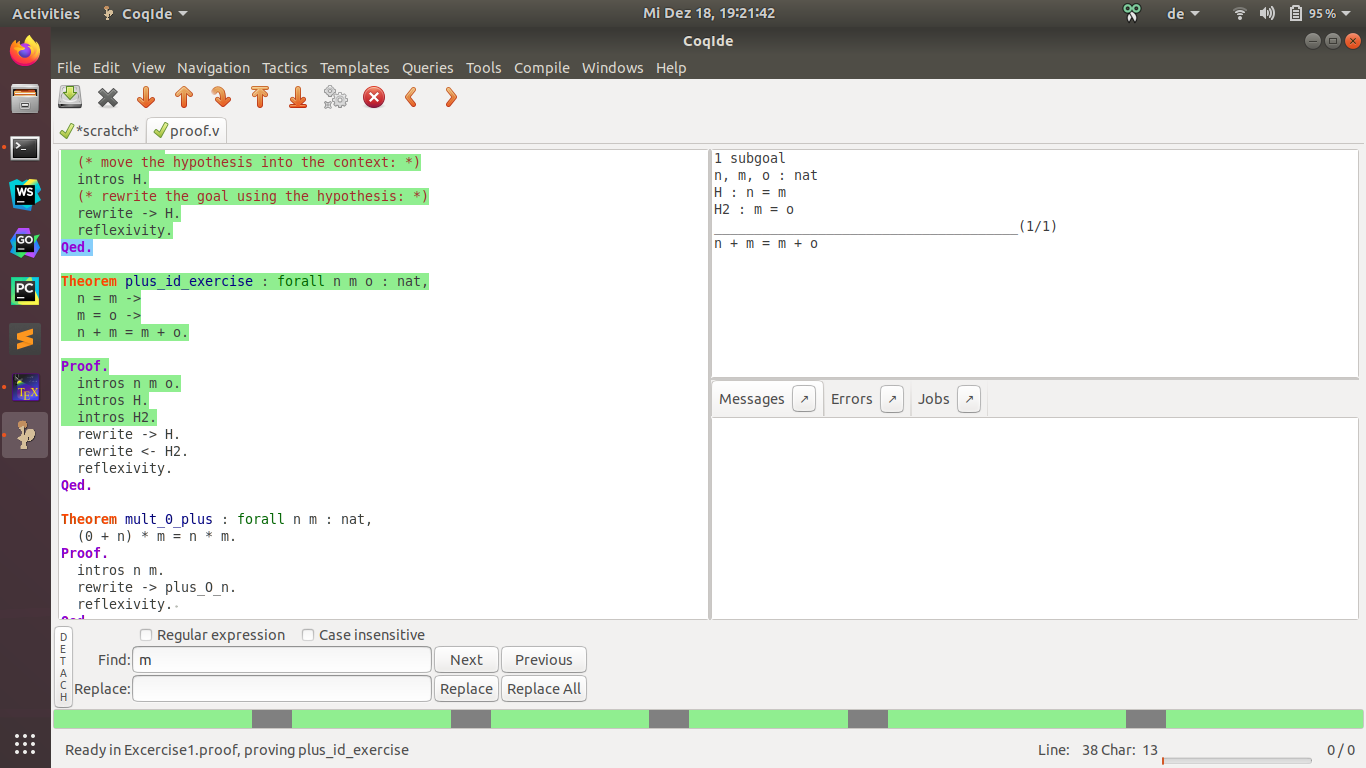
\includegraphics[width=1\textwidth]{\figdir/Coqide-sample.png}
	\caption{Coqide}
	\label{fig:coqide-sample}
\end{minipage}
Die Coqide bietet viele spezielle Features für formale Verifikation. Beispielsweise ist es möglich mit den Pfeilen in der Navigationsleiste die einzelnen Kommandos aus der linken Textbox auszuführen. Je nach Pfeil springt man einen Schritt vorwärts, bis zum Zeiger vorwärts oder auch rückwärts.\\
\\
Die Entwicklungsumgebung stellt grundsätzlich drei Fenster dar. Dabei wird eines für den Programmcode genutzt. Die anderen beiden Fenster auf der rechten Seite dienen ausschließlich der Informationsausgabe.\\
Im Screenshot ist ein Beweis zu sehen. Dabei wird überprüft, wenn die natürlichen Zahlen \textbf{n, m, o} und die Beziehungen \textbf{n = m} und \textbf{m = o} gegeben sind, dass \textbf{n + m = m + o} gilt.\\
Zunächst fällt auf, dass der Coq-Code teilweise grün markiert ist. Dies symbolisiert den bereits erfolgreich ausgeführten Teil. Das Ausgabefenster rechts oben zeigt, hierfür die passende Ausgabe. Dabei werden über dem Trennstrich die gegebenen Zahlen und Hypothesen angezeigt. Zusätzlich ist noch die Anzahl an Zielen abgebildet. Den darunter stehende Ausdruck gilt es zu beweisen.\\
Das dritte Fenster rechts unten dient zur Meldung von Hinweisen, Fehlern und Konsolenausgaben, wie beispielsweise von einer Suche.\\
\\
Im Anschluss folgt das bereits gezeigte Codebeispiel \ref{lst:sample-proof2} mit der ausführlichen Ausgabe der Coqide nach jedem Schritt.
Diese ist durch die Kommentarblöcke, welche durch \textbf{(*} eingeleitet und durch \textbf{*)} beendet werden, gekennzeichnet.
Wie bereits zuvor erklärt, gilt es, unter den gegebenen Umständen, \textbf{n + m = m + o} zu beweisen. Hierfür wird die \textbf{rewrite} Taktik eingesetzt. Nicht fachlich ausgedrückt bedeutet es, dass je nach Richtung des Pfeils die eine oder die andere Seite eingesetzt wird. Somit verändert sich die zu beweisende Aussage dynamisch im Coqide-Ausgabefeld. Nach dem ersten \textbf{Rewrite}, wird \textbf{n} mit \textbf{m} ersetzt. Das Einsetzen der zweiten Hypothese \textbf{H2} führt schlussendlich zu dem Ergebnis: \textbf{m + m = m + m}. Folglich kann das Ziel mit \textbf{reflexivity} bewiesen werden.
\begin{lstlisting}[language=coq,firstnumber=1,caption=Coq Beispielbeweis,label=lst:sample-proof2]
(* Initiating the theorem to proof. *)
Theorem plus_id_exercise : forall n m o : nat,
	n = m ->
	m = o ->
	n + m = m + o.
	
(* result: 
1 subgoal
______________________________________(1/1)
forall n m o : nat,
n = m -> m = o -> n + m = m + o*)

Proof.
(* move quantifiers into the context: *)
	intros n m o. 
	
(* result: 
1 subgoal
n, m, o : nat
______________________________________(1/1)
n = m -> m = o -> n + m = m + o*)

(* move hypothesises into the context: *)	
	intros H.
	intros H2.

(* result: 
1 subgoal
n, m, o : nat
H : n = m
H2 : m = o
______________________________________(1/1)
n + m = m + o*)

(* rewrite the goal using the hypothesises: *)
	rewrite -> H.

(* result: 
...
______________________________________(1/1)
m + m = m + o
*)
	rewrite <- H2.

(* result:
...
______________________________________(1/1)
m + m = m + m
*)
	reflexivity.
Qed.
\end{lstlisting}

\section{Coq und Programmcode}
\label{s:coq-and-code}

Beim Zusammenspiel von Beweisen in Coq und Programmcode gibt es zwei verschiedene Richtungen. Einerseits können Theoreme bewiesen und dann in Programmiersprachen extrahiert werden. Andererseits ist es auch möglich, erst ein Programm zu entwickeln und anschließend dieses in Coq zu verifizieren. \\
Das dabei verwendete Prinzip lautet vereinfacht gesagt:
\textbf{Es gibt eine Liste von Dingen, die eine Software tun soll. Hierfür wird Logik verwendet, um zu beweisen, dass diese Software auch genau diese Dinge tut.}
\\
In den folgenden Unterkapiteln sind beide Wege beschrieben. Dabei wird die Richtung Proof zu Programm anhand eines genauen Codebeispiels erläutert.

\subsection{Proof -> Programm}
\subsubsection{theoretisch}
{Wie bereits zuvor erwähnt, ist der erste Schritt die Erstellung einer Spezifikation, welche die Software beschreibt. Anschließend muss diese in mathematischer Form in ein Proof Tool geschrieben und bewiesen werden. Auf fehlerhafte Beweise weißt dieses Tool hin.
Sobald jetzt ein Fehler in der realen Welt auftritt, sollte dieser mit diesem beschrieben Model abgefangen werden. \\
Schlussendlich müssen die bewiesenen Anforderungen der Spezifikation in Programmcode konvertiert werden. Dieser Prozess wird in folgendem Kapitel genauer erklärt.}\cite{HELWER01:FV}

\subsubsection{praktisch}
In diesem Kapitel wird erklärt, wie Funktionen formal mit Coq bewiesen werden und anschließend in Ocaml extrahiert und ausgeführt werden. Ocaml ("`Categorical Abstract Machine + ML"') ist eine sowohl funktionale, als auch objektorientierte Programmiersprache. ML bedeutet Meta-Language. Dies ist allerdings für diese Arbeit weniger relevant, da Ocaml lediglich als Beispiel für Code-Extraktion genutzt wird. Der Fokus dieser Arbeit liegt auf dem Prinzip und nicht auf einer speziellen Programmiersprache.\\
Bei dem Ansatz von Proof zum Programmcode musst zu Beginn eine \textbf{.v}-Datei erstellt werden. Darin wird der Coq-Code geschrieben. Das verwendete Beispiel \ref{lst:practical-functions} stellt ein Datentyp Paar von natürlichen Zahlen dar. Hierfür sollen verschiedenste Funktionalitäten implementiert werden. Dabei sind Funktionen wie \textbf{fst}, \textbf{snd} und \textbf{swap\_pair}. Anschließend sind Beweise, die verschiedenste Eigenschaften der einzelnen Funktionen prüfen, dargestellt.

\begin{lstlisting}[language=coq,firstnumber=1,caption=Coq Funktionen für Paare aus natürlichen Zahlen,label=lst:practical-functions]
From LF Require Export Induction.

Inductive natprod : Type :=
	| pair (n1 n2 : nat).

Check (pair 3 5).

Definition fst (p : natprod) : nat :=
match p with
	| pair x y => x
end.

Definition snd (p : natprod) : nat :=
match p with
	| pair x y => y
end.

Compute (fst (pair 3 5)).
Compute (snd (pair 5 7)).

Notation "( x , y )" := (pair x y).

Compute (fst (3,5)).

Definition swap_pair (p : natprod) : natprod :=
match p with
	| (x,y) => (y,x)
end.
\end{lstlisting}
Zu Beginn wird der \textbf{induktive Typ natprod} definiert, welcher ein Paar repräsentiert. Im darauf folgenden Teil des Codebeispiels werden immer wieder die Schlüsselwörter \textbf{Check} und \textbf{Compute} verwendet. Mit Hilfe dieser Funktionen können stichprobenartig einzelne Werte in die Definitionen oder Typen eingesetzt werden. Anschließend wird das daraus resultierende Ergebnis ausgegeben.\\
Die Funktionen \textbf{fst} und \textbf{snd} geben jeweils x oder y eines Paares zurück. Weiterhin ist eine Notation für die Definition von Paaren dargestellt. Diese dient ausschließlich dafür, dass anstelle von 
\textbf{(pair x y)} auch \textbf{(x , y)} verwendet werden darf. Wenn eine solche Notation nicht vorhanden wäre, müsse eine komplett neue Funktion \textbf{fst'} für den Syntax von \textbf{(x , y )} geschrieben werden. Notationen sind prinzipiell Aliase und tragen zur Kürzung des Aufwands bei.\\
Zuletzt wird die \textbf{swap\_pair} Funktion, die den X- und Y-Wert eines Paares vertauscht zurückgibt, definiert.\\
\\
Anschließend müssen Eigenschaften die diese Funktionen erfüllen sollen, bewiesen werden.
Zuerst wird mit Hilfe der Theoreme surjective\_pairing und surjective\_pairing\_stuck bewiesen, dass das Erstellen von einem neuem Paar demselben entspricht, wenn man fst und snd von diesem Paar nimmt und somit ein neues Paar bildet. Die zwei Funktionen unterscheiden sich lediglich in der Verwendung des Syntax von Paaren. Bei surjective\_pairing\_stuck wird außerdem die \textbf{destruct} Taktik benötigt.\\
Diese teilt normalerweise das Hauptziel des Beweises in die einzelnen Subgoals \textbf{n = O} und \textbf{n = S n'} auf. Sobald beide Ziele bewiesen wurden, akzeptiert Coq dieses Theorem. Hierbei ist der Unterschied zur Induktion, dass dabei \textbf{n = 0, n + 1} gecheckt wird und anschließend die Schlussfolgerung auf Korrektheit möglich ist.\\
Im Beispiel wird \textbf{destruct} jedoch nur zur Aufteilung von \textbf{p} in die natürlichen Zahlen n und m verwendet.
Ab dieser Zeile entspricht dieser Beweis exakt dem Ersten, welcher von Anfang an natürliche Zahlen verwendet. 

\begin{lstlisting}[language=coq,firstnumber=1,caption=Coq Beweise für Paar Funktionen,label=lst:practical-proof]
Theorem surjective_pairing' : forall (n m : nat),
(n,m) = (fst (n,m), snd (n,m)).
Proof.
	simpl.
	reflexivity. 
Qed.

Theorem surjective_pairing_stuck : forall (p : natprod),
p = (fst p, snd p).
Proof.
	intros p.
	destruct p as [n m].  
	simpl.
	reflexivity.
Qed.

Theorem snd_fst_is_swap : forall(p : natprod),
(snd p, fst p) = swap_pair p.
Proof.
	intros p.
	destruct p as [n m].
	simpl.
	reflexivity.
Qed.

Theorem fst_swap_is_snd : forall(p : natprod),
fst (swap_pair p) = snd p.
Proof.
	intros p.
	destruct p as [n m].
	simpl.
	reflexivity.
Qed.
\end{lstlisting}

Die nächsten zwei Theorem prüfen bestimmte Eigenschaften der \textbf{swap\_pair} Funktion. Zuerst wird Bewiesen, dass das zweite Element eines Paares in Verbindung mit dem ersten, das Ergebnis der Definition \textbf{swap\_pair} ist. Letzterer Beweis stellt sicher, dass für jeden \textbf{natprod} das erste Element eines Paares nach einem Aufruf von \textbf{swap\_pair} dem ursprünglich zweiten Wert des Paares entspricht.\\
Beide Theoreme werden identisch zu surjective\_pairing\_stuck bewiesen. Dabei wird der \textbf{natprod}-Typ ebenfalls mit Hilfe von \textbf{destruct} in zwei natürliche Zahlen aufgeteilt.\\
\\
Um anschließend die formal bewiesenen Funktionen in Programmen nutzen zu können, muss die Datei, in der die Beweise geschrieben wurden, in Coq compiliert werden. Dafür muss folgender Befehl in die Kommandozeile eingeben werden:
\textbf{coqc -Q . LF PaperPair.v}. \\
\textbf{Coqc} ist hierbei der Aufruf des Coq-Compilers. \textbf{-Q . LF} sorgt dafür, dass alle .v-Dateien aus dem Paket LF in andere Coq-Dateien importiert werden können. Ein Paket in Coq ist ähnlich zu anderen Programmiersprachen wie beispielsweise Java.
\\
Für den nächsten Schritt in der Extraktion wird eine Coq-Datei benötigt, welche definiert, wie und was in welcher Sprache extrahiert werden soll. Diese muss ebenfalls über die Kommandozeile, wie zuvor beschrieben, compiliert werden.
\begin{lstlisting}[language=coq,firstnumber=1,caption=Coq Code extrahieren,label=lst:practical-proof-extraction]
Require Extraction.
Extraction Language OCaml.
Require Import ExtrOcamlBasic.
Require Import ExtrOcamlString.
Require Import Arith Even Div2 EqNat Euclid.

Extract Inductive nat => int [ "0" "Pervasives.succ" ]
"(fun fO fS n -> if n=0 then fO () else fS (n-1))".

Extraction "paperimpl.ml" fst snd swap_pair.
\end{lstlisting}
Im Codeblock \ref{lst:practical-proof-extraction} ist zu sehen, dass verschiedene Dateien mit \textbf{Require} und \textbf{Require Import} importiert werden. \textbf{Extraction} und \textbf{ExtraOcamlBasic} sind beispielweise Standard-Features von Coq um Funktionen von Coq-Code in Ocaml-Code umzuwandeln.\\
Weiterhin wird in der Zeile \textbf{Extract Inductive nat => \dots} ein Ausdruck verwendet, sodass OCaml den Typ der natürlichen Zahlen aus Coq verwenden kann. Allerdings ist der Coq-Code zu Ocaml Extraktor nicht formal verifiziert. Die Korrektheit wird trotzdem angenommen, da Coq großteils Ocaml geschrieben ist.
Damit schlussendlich eine ausführbare Datei entsteht, muss definiert werden, welche Funktionen in welche Datei extrahiert werden sollen.\\
\\
Der folgende Code \ref{lst:practical-generated-code} ist das Resultat, des zuvor gezeigten Coq-Codes. 
\begin{lstlisting}[language=coq,firstnumber=1,caption=Ocaml Code anpassen,label=lst:practical-generated-code]
type natprod =
| Pair of int * int

(** val fst : natprod -> int **)

let fst = function
| Pair (x, _) -> x

(** val snd : natprod -> int **)

let snd = function
| Pair (_, y) -> y

(** val swap_pair : natprod -> natprod **)

let swap_pair = function
| Pair (x, y) -> Pair (y, x)
\end{lstlisting}
Dadurch das der Coq-To-Ocaml-Extraktor nicht komplett formal verifiziert ist, kann es sein, dass der Code nicht 100\% korrekt ist. Um sicherzustellen, dass dies der Fall ist, wurden im Nachhinein ein paar Tests geschrieben, welche im Codebeispiel \ref{lst:practical-code-adjustment} dargestellt werden. Diese Tests beschreiben einfache Funktionsaufrufe wie zum Beispiel das Erhalten des ersten und zweiten Wertes eines Paares. Anschließend werden die selben Funktionen noch einmal aufgerufen - allerdings auf ein neues Paar, dass du die swap\_	pair Funktion entstanden ist. Zur Nachvollziehbarkeit werden dabei die jeweiligen Ergebnisse auf der Kommandozeile ausgegeben.
\begin{lstlisting}[language=coq,firstnumber=1,caption=Ocaml Code anpassen,label=lst:practical-code-adjustment]
let pair = Pair(3, 4);;
let resultfst = fst pair;;
let resultsnd = snd pair;;

Printf.printf "Result fst: %d \n%!" resultfst;;
Printf.printf "Result snd: %d \n%!" resultsnd;;

let pair2 = swap_pair pair;;
let resultfst2 = fst pair2;;
let resultsnd2 = snd pair2;;

Printf.printf "Result fst: %d \n%!" resultfst2;;
Printf.printf "Result snd: %d \n%!" resultsnd2;;
\end{lstlisting}
Ocaml-Code muss genauso wie C-Code compiliert werden. Folgender Befehl ermöglicht es aus der \textbf{paperimpl.ml} und der \textbf{paperimpl.mli} Datei funktionierenden compilierten Code zu erhalten. Dieser wird unter dem Namen \textbf{paperimp} im selben Verzeichnis abgelegt.
\\
\begin{lstlisting}[language=coq,firstnumber=1,caption=Ocaml Code compilieren,label=lst:practical-code-compilation]
ocamlc -w -20 -w -26 -o paperimp paperimpl.mli paperimpl.ml
\end{lstlisting}

\begin{lstlisting}[language=coq,firstnumber=1,caption=Ocaml code ausführen,label=lst:practical-code-execution]
lukas@luk-ubuntu@~/Documents/coq-test/lf: ./paperimp
Result fst: 3 
Result snd: 4 
Result fst: 4 
Result snd: 3 
\end{lstlisting}
In Codeblock \ref{lst:practical-code-execution} werden die Ausgaben der Tests dargestellt. Die ersten zwei Ergebnisse sind die Werte, welches mit den Werten \textbf{fst: 3} und \textbf{snd: 4} initiiert wurde. Die zweiten zwei Ausgaben stellen \textbf{fst} und \textbf{snd} des invertierten Paars dar.

\subsection{Programm -> Proof}
Generell ist es möglich fast jeden Programmcode formal zu verifizieren. Der Aufwand, der dafür aufzubringen ist, unterscheidet sich gewaltig. Um den Code einer Sprache vollständig formal beweisen zu können, muss theoretisch auch der Compiler der Sprache formal bewiesen sein. Ansonsten wäre zwar der Programmcode formal verifiziert, allerdings kann nicht garantiert werden, dass der Compiler dennoch Fehler beim übersetzen macht. Des Weiteren ist noch zu erwähnen, dass der Compiler nicht die niedrigste Software-Ebene repräsentiert. In den Schichten darunter sind beispielsweise noch Hardwarebeschreibungssprachen. Sobald dort ein gravierender Bug enthalten ist, kann der high-level Programmcode formal bewiesen sein und trotzdem fehlerhaft laufen.\\
\\
\subsubsection{Beispiel Programmiersprache C}
Der Code aus der Programmiersprache C wird zum Beispiel in Maschinencode umgewandelt. 
Um diese Konvertierung durchführen zu können, haben Forscher von INRIA und der Princeton University die Verified Software Toolchain (VST), oder auch Princeton Tool Chain genannt, entwickelt. Auf folgender Illustration \ref{fig:vst} sind die einzelnen Komponenten von der VST abgebildet. Zuerst wird dabei das C-Source-Programm in Verifiable C übersetzt. \\
"`Verifiable C ist grundsätzlich korrekt. Das heißt, es ist nachgewiesen (mit einem maschinell geprüften
Beweis im Coq-Proof-Assistenten), dass:\\
\textbf{Egal welche beobachtbare Eigenschaft eines C-Programms Sie auch immer beweisen wollen. Unter Verwendung der Verifiable C-Programmlogik, wird diese Eigenschaft
tatsächlich im Assemblerprogramm enthalten sein, welches der C-Compiler generiert.}"'\\
Mit \textbf{program logic} ist eine Art Hoare Logik gemeint, die ein leichteres Beweisen von Programmcode mit Pointern, Funktions-Pointern, Datenabstraktion und Datenstrukturen ermöglicht.\cite{Appel02:VST} Die Hoare Logik wurde durch den britischen Informatiker C. A. R. Hoare entwickelt und dient generell als Hilfsmittel für das Beweisen von Programmcode. Dabei werden logische Regeln aufgestellt, die es erlauben, Aussage in mathematischer Form über Computer-Programme zu treffen.\\
Die in orange dargestellte Komponente bezüglich der \textbf{VST retargetable Seperation Logic} ergänzt die \textbf{program logic}. Außerdem können dadurch zusätzliche \textbf{verified program analysis tools} integriert werden.\\
\\
Der nächste Schritt in der Princeton Tool Chain ist der \textbf{verified Compiler CompCert}. Dieser wurde von INRIA entwickelt und ist wie die VST open-source auf GitHub erhältlich unter \url{https://github.com/PrincetonUniversity/VST} und \url{https://github.com/PrincetonUniversity/VST/tree/master/compcert}. 
CompCert wandelt schlussendlich den Verifiable C Code in Maschinensprache um.

\begin{minipage}{\textwidth}
	\centering
	\captionsetup{type=figure}
	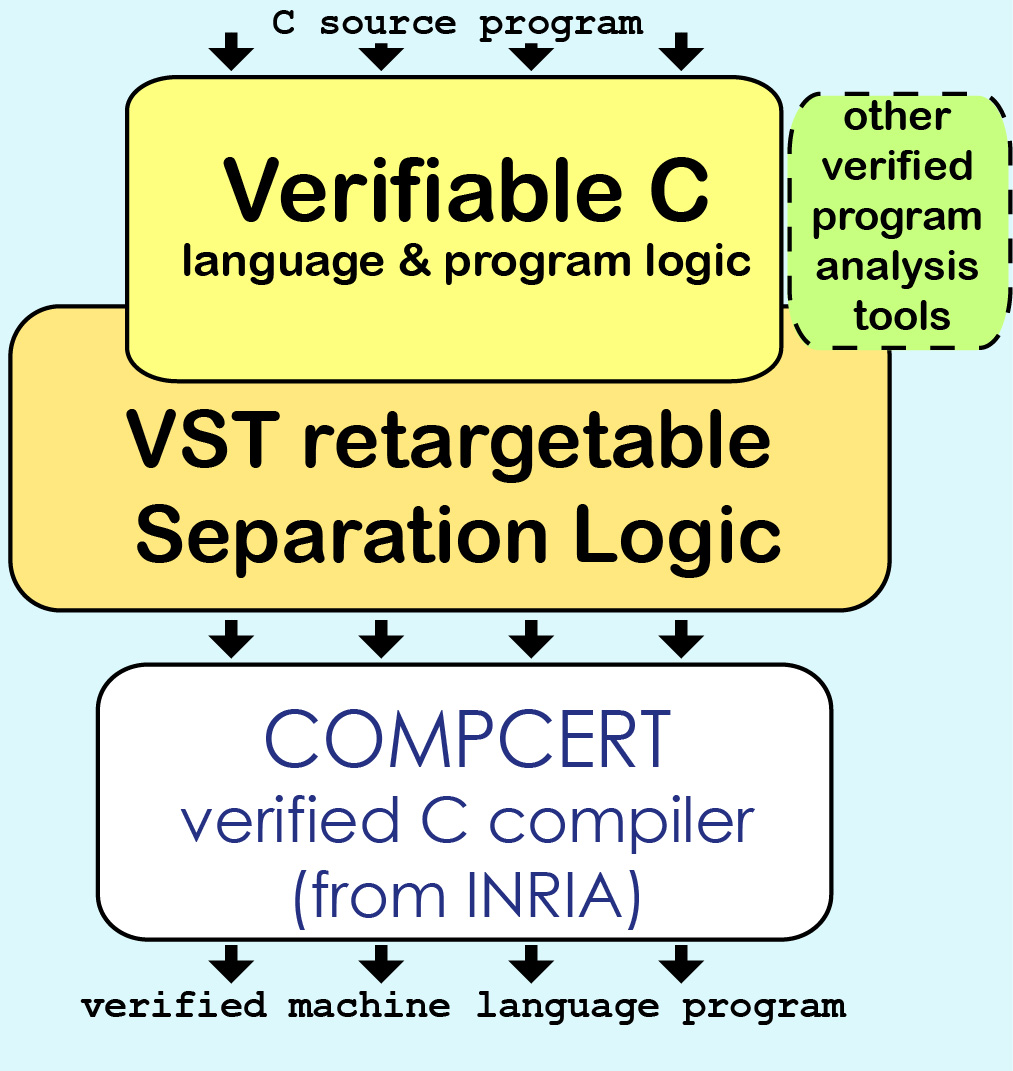
\includegraphics[width=0.6\textwidth]{\figdir/VST-diagram.jpg}
	\caption{Verified Software Toolchain\cite{PRINCETON01:VST}}
	\label{fig:vst}
\end{minipage}

\subsubsection{Wie benutzt man die VST?}
Im vorherigen Unterkapitel wurde erklärt, aus welchen Komponenten die Princeton Tool Chain besteht. Der Compiler CompCert ist dabei bereits komplett formal verifiziert. Dies bedeutet, dass jeder in verifiable C geschriebene Programmcode in den entsprechenden Assemblercode übersetzt wird. Es stell sich die Frage, wie und wo die selbstgeschriebenen Funktionen auf mathematische Korrektheit geprüft werden.\\
\\
{Hierfür wird aus dem Paper "´\textbf{Verifiable C} Applying the Verified Software Toolchain to C programs"' das Vorgehen beschrieben.\\
Zuerst muss ein C-Programm in eine Datei \textbf{F.c} geschrieben werden. Anschließend muss der normale C-Code in Verifiable C übersetzt werden. Dies ist mit Hilfe des Command Line Interface (CLI) Kommandos \textbf{clightgen -normalize F.c} möglich. Dadurch entsteht eine Coq-Datei \textbf{F.v}. Um die darin stehenden Funktionen zu beweisen, muss eine Datei mit beispielsweise dem Name \textbf{verif\_F.v} erstellt werden. Wichtig dabei ist, dass in der Datei sowohl \textbf{F.v} als auch das VST Floya Programm-Verifikationssystem \textbf{VST.floyd.proofauto} importiert werden. Wenn ein Beweisen aller Funktionen gelingt, ist das C-Programm korrekt geschrieben und somit maschinell formal verifiziert.}\cite{Appel01:VST}


\section{Aktuelle Anwendung}
\label{s:current-usage}
In diesem Kapitel werden ein paar neben der Princeton Toolchain existierenden Anwendungsfälle und Projekte aufgeführt und kurz vorgestellt.

\subsection{Proofed Stack}
Mit Hilfe von VST inklusive CompCert wird versucht eine Art Stack aufzubauen, der von Maschinensprache über das Betriebssystem bis hin zu C-Programmcode formal verifiziert ist. Hierfür wird zusätzlich ein spezielles Coq-Framework namens \textbf{Kami} verwendet. Damit ist es möglich Hardware-Design formal zu beweisen. Diese Domain specific Language (DSL) ist hauptsächlich inspiriert von \textbf{Bluespec} und der open-source \textbf{RISC-V} Befehlssatzarchitektur.\cite{KAMI01:ST} Vereinfacht gesagt, beschreibt dies die Verhaltensweise eines Prozessors in Form von einer formalen Spezifikation.\\
Die zur Architektur passenden Chips werden beispielsweise durch \textbf{SiFive}, welche auch \textbf{Kami} entwickelt haben, hergestellt.\\
Schlussendlich fehlt noch ein Betriebssystem, welches zum ein oder anderen Zeitpunkt mit Prozessoren und Speichern interagiert. Hierfür wurde \textbf{CertiKOS}, das erste formal verifizierten Betriebssystem, entwickelt. Es unterstützt \textbf{x86} inklusive Multiprozessing. Außerdem ist es möglich, einen Hypervisor zu hosten und dadurch mehrere Betriebssysteme gleichzeitig auf der selben Maschine zu verwenden.\cite{CERTIKOS01:FV}\cite{CERTIKOS02:FV}\\
\\
Der ganze proof Stack könnte ungefähr wie in der folgenden Illustration \ref{fig:proofed-stack} dargestellt werden. Dabei wird Hardware-Komponenten in rot markiert. Der Softwareteil wird farblich unterschiedlich abgebildet mit dem Ziel, dass das Bild übersichtlicher ist.\\


\begin{minipage}{\textwidth}
	\centering
	\captionsetup{type=figure}
	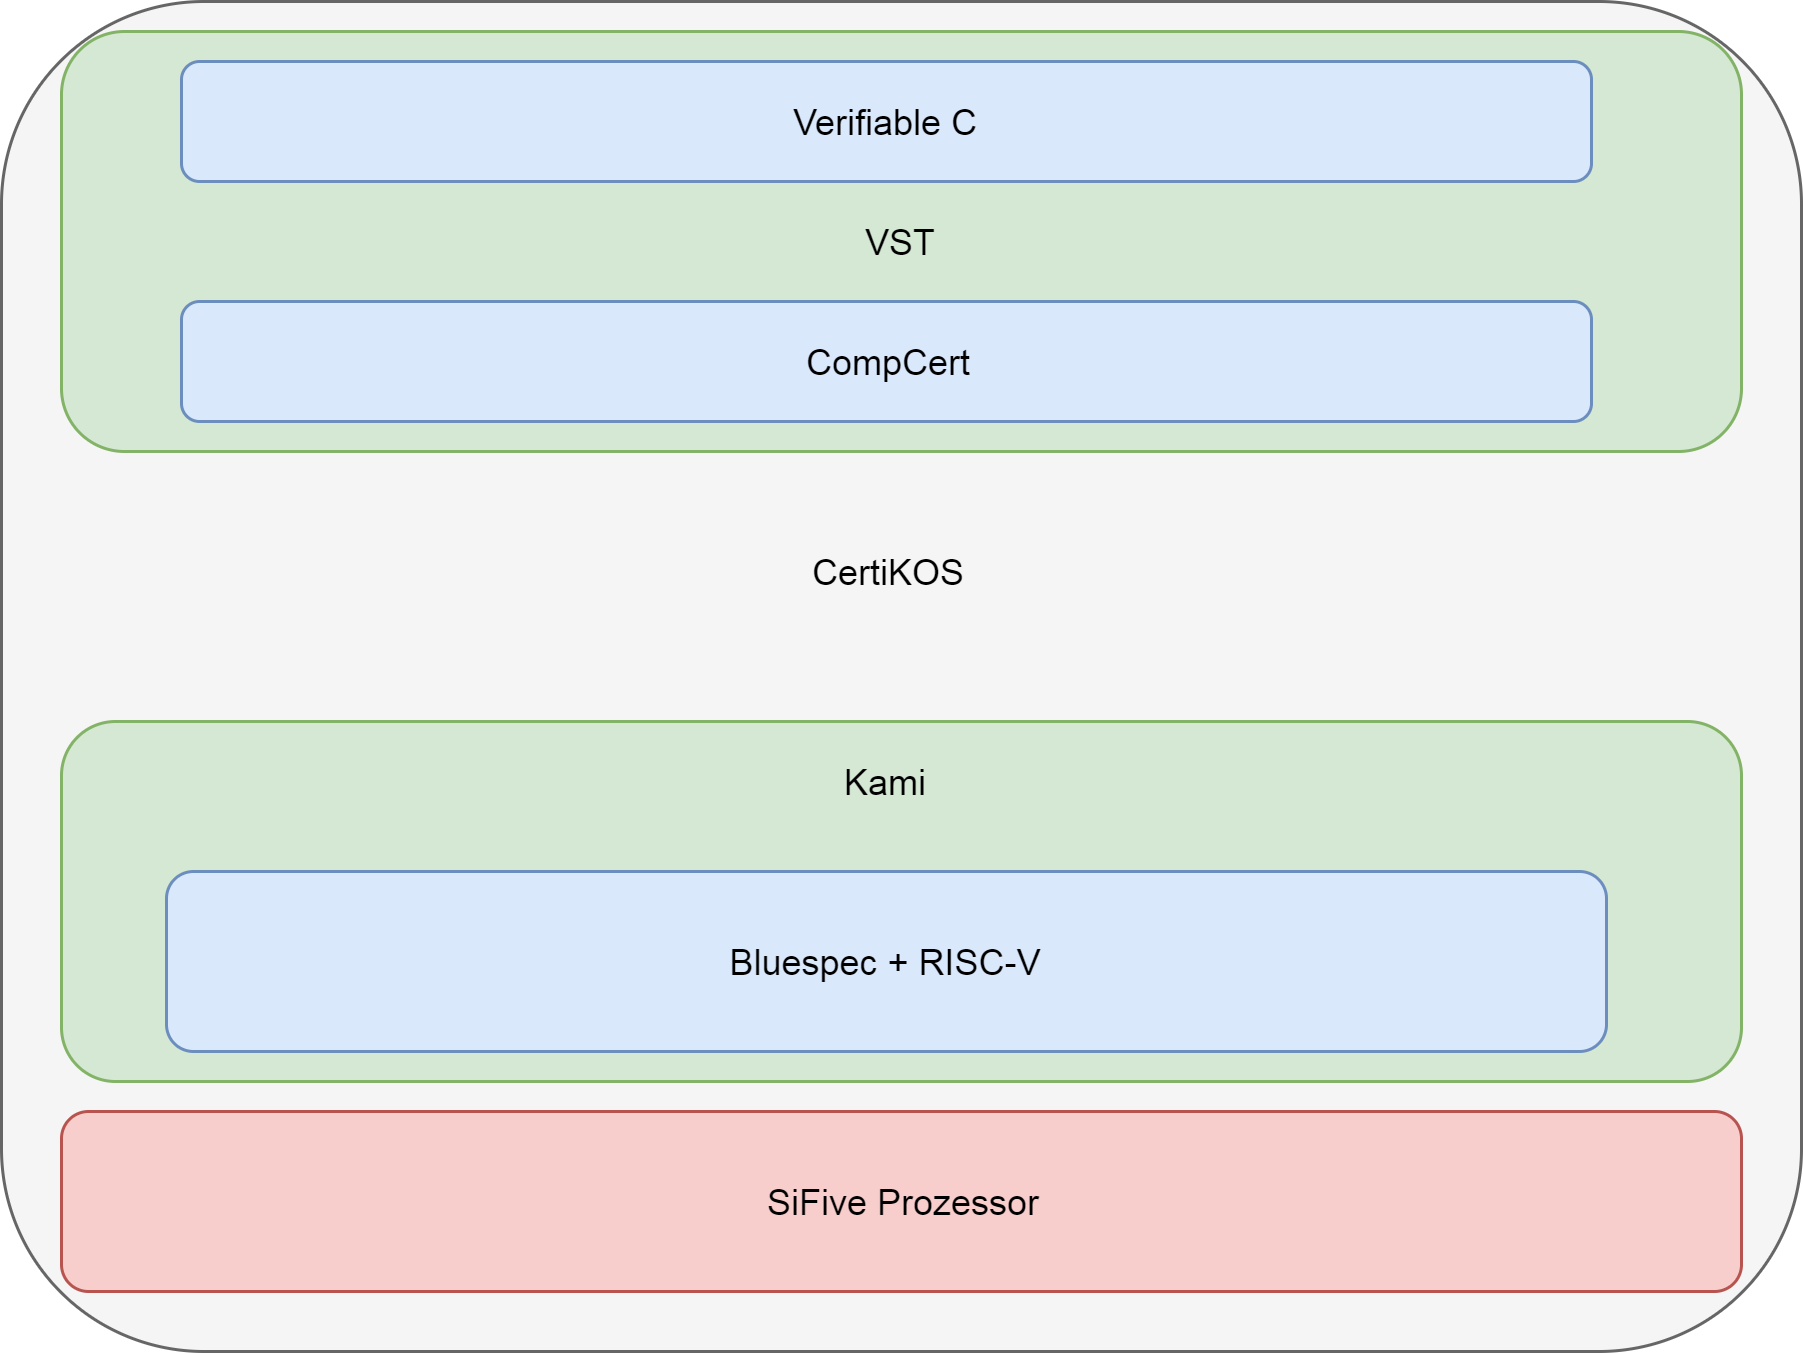
\includegraphics[width=0.6\textwidth]{\figdir/verified-stack.png}
	\caption{Proofed Stack}
	\label{fig:proofed-stack}
\end{minipage}


\subsection{JSCert}
JSCert ist eine maschinell in Coq geprüfte Spezifikation von JavaScript. Es wurde mit der Coq Version 8.4.6 geschrieben. Dabei wurde versucht sich so nah wie möglichst am englischen Standard ECMAScript 5 zu halten. Damit wurde ein Ocaml geschriebener Interpreter namens \textbf{JSRef} als korrekt bewiesen. Dabei wurden 262 Testfälle abgedeckt.\cite{JSCERT01:FV}\cite{JSCERT012:FV}

\subsection{CertiCoq}
CertiCoq ist ein in Coq verifizierter Compiler für Coq. Genauer genommen beweist CertiCoq, dass die Compilierung von typ-abhängigen Sprachen, wie Gallina korrekt verläuft.\cite{CERTICOQ01:FV}\cite{CERTICOQ02:FV} Weitere Informationen diesbezüglich sind auf der Website der Princeton University zu finden.

\subsection{Beweise für Probleme der Mathematik oder Informatik}
Mit Coq kann nicht nur Programmcode verifiziert werden. Die Grundlage dafür sind schließlich mathematische Beweise inklusive Taktiken und der interaktiven Entwicklungsumgebung. Somit wird Coq auch von Theoretikern, welche vor allem aus den Fachbereichen der Mathematik und Informatik kommen, genutzt. Die folgenden zwei bekannten Probleme wurden mittels Coq bewiesen. 

\subsubsection{Satz von Feit-Thompson}
Das Odd-Order-Theorem, zu deutsch Satz von Feit-Thopmson sagt aus, dass jede endliche Gruppe von ungeraden Ordnungen auflösbar ist. Dies wurde bereits durch Walter Feit und John Griggs Thompson 1963 bewiesen.\\
Nach einer sechsjährigen Arbeit gelang Georges Gonthier von INRIA 2012 die Verifikation in Coq. Dies wurde als Forschung-Projekt zur Weiterentwicklung von Coq durchgeführt. Dabei sind über 150000 Zeilen an Beweis-Code entstanden, welche circa 4000 Definition und 13000 Theoreme enthalten.\cite{ODD01:FV}

\subsubsection{Vier-Farben-Theorem}
Das Vier-Farben Theorem sagt aus, dass es immer möglich ist, mit Hilfe von vier Farben eine beliebige Landkarte in der euklidischen Ebene einzufärben. Dabei dürfen angrenzende Länder niemals gleich gefärbt sein. Weiterhin werden isolierte gemeinsame Punkte nicht als Grenze gewertet. Eine weitere Einschränkung ist, dass keine Exklaven vorhanden sein dürfen. Dies bedeutet, dass die Karte aus einer zusammenhängenden Fläche bestehen muss(siehe Grafik \ref{fig:four-color}).\cite{FOURCOLORS01:FV}\\
Im Jahr 2005 wurde dieses Theorem erstmals durch die zwei Forscher Goerges Gonthier und Benjamin Werner vollständig mit Coq bewiesen.
\cite{FOURCOLORS02:FV}\\

\begin{minipage}{\textwidth}
	\centering
	\captionsetup{type=figure}
	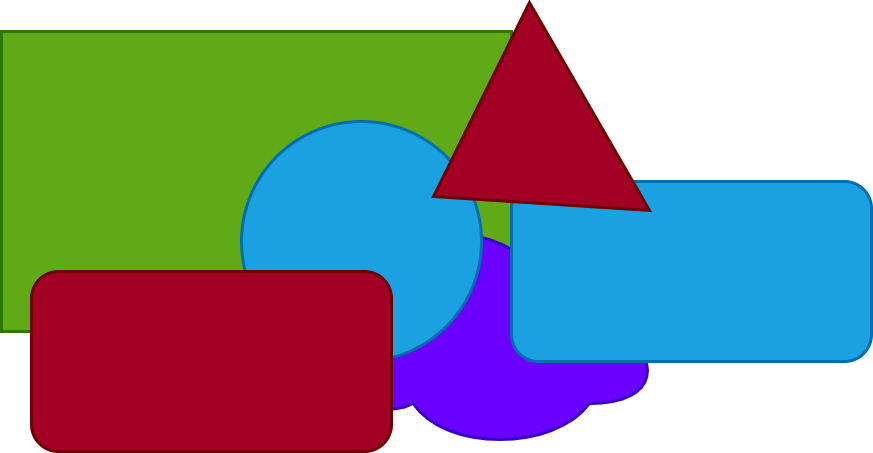
\includegraphics[width=0.3\textwidth]{\figdir/four-color.png}
	\caption{Beispiel für Vier-Farben-Problem}
	\label{fig:four-color}
\end{minipage}

\section{Aufwand in der Praxis}
Der Aufwand für formale Verifikation ist schwer abzuschätzen, da diese Art von Programmieren nicht für jedes Teilgebiet gleichmäßig erforscht ist oder überhaupt benötigt wird. Grundsätzlich nutzen vor allem große Firmen im Bereich der low-level Software diese Form der Verifizierung. Damit kann sichergestellt werden, dass der Prozessor immer korrekt angesteuert wird et cetera. Dabei werden meist funktionale Sprachen, wie beispielsweise C oder maschinennahe Sprachen verwendet. Dem entsprechenden, ist in diesen Bereichen die Forschung bereits sehr weit vorgedrungen im
Vergleich zu anderen Programmiersprachen wie Java oder C\#.\\
\\
In einem Talk über das Projekt Ironclad von Microsoft Research sprach Bryan Parno 2014 über den Vorgang beim Einsetzen von Formaler Verifikation bei einer Ende-zu-Ende Sicherheits-Anwendung. Dabei nannte benannte er den Aufwand für das Programmieren mit etwa fünft Zeilen extra Beweis-Code pro richtiger Zeile Code. Außerdem sei es eine komplett neue Art zu Software zu entwickeln. Abschließend fügte er noch hinzu, dass der meiste neue Code "`out-of-the-box"' funktionierte und faktisch kaum Bugs enthielt.\cite{IRONCLAD01:FV}

\section{Fazit}
\begin{itemize}
	\item \url{https://medium.com/background-thread/the-future-of-programming-is-dependent-types-programming-word-of-the-day-fcd5f2634878}
	\item Programmcodeverifikation nimmt vor allem in sicherheitskritischen Bereichen zu
	\item Programmcodeverifikation ist deutlich zeitintensiver (5mal)
	\item Mit dieser Verifikation kann 100\%tige Garantie für funktionierende Software gewährleistet werden. Weil Assertions bereits zu Compilezeit durchgeführt werden und nicht mehr zur Laufzeit.
	\item Es hat großes Potential
	\item Wird sehr stark durch die Community weiterentwickelt
	\item Große Firmen nutzen es immer aktiver
	\item nur Software kann sicher gemacht werden. Hardware ist immer noch fehlbar!
\end{itemize}

\section{Glossar}


%%% Local Variables: 
%%% mode: latex
%%% TeX-master: "thesis.tex"
%%% End: 
